\chapter{Solución propuesta}

    En este cápitulo, comentaremos la solución que hemos propuesto, y que
    hemos llevado a cabo para conseguir una autenticación a través de la
    federación de identidad para SSH.

    \section{Posibles soluciones barajadas}

    La parte más importante de este proyecto es la conexión entre la
    federación de identidad, basada en aplicaciones web, y los servidores
    SSH.

    Para conseguir esta conexión, es casi imprescindible una pequeña
    aplicación web, que esté tras un proveedor de servicio, y la cual pueda
    acceder a los atributos del usuario, una vez este se haya autenticado
    en el IdP de su organización.

    Esta aplicación web, será la que diga si un usuario está
    autenticado en la federación o no, y su funcionamiento variará
    ligeramente, según la implementación concreta de la solución.

    \textbf{Servidor ssh}:

    Como primera opción se barajó la idea de utilizar un modulo PAM
    (Plugable Authentication Method), ya que el servidor SSH permite este
    tipo de autenticación. Los módulos PAM son un método que permite al
    administrador controlar cómo se realiza el proceso de autenticación de
    los usuario para aplicaciones, a través de unas bibliotecas.

    La opción de los módulos PAM permitiría el acceso sin tener que tocar
    el servidor SSH, sino simplemente añadiendo un módulo al sistema, y
    cambiando una línea en un fichero de configuración.

    Pero como inconveniente tiene que estos módulos autentican con usuario
    y contraseña, por lo que o se le pasa el usuario y contraseña al
    servidor SSH (cosa que no queremos), o se crea una cuenta de un solo
    uso.

    Otra posible solución es utilizar el método de autenticación por clave
    pública que proporciona el servidor openssh. Este método permite
    autenticar a un usuario sin que este tenga que introducir su
    contraseña, y sería lo más automático posible.

    Este método funciona buscando la clave pública del usuario en un
    fichero del sistema local. Pero nosotros no tenemos un fichero en cada
    servidor SSH con las claves de los usuarios autenticados. Además esta
    lista de usuarios será dinámica.

    La solución que hemos elegido para solventar el problema es la segunda,
    pero es necesario que además de mirar en los ficheros locales, pregunte
    a un servidor intermedio, para saber qué usuarios están autenticados en
    la federación. Para esto es necesario tocar un poco el código del
    servidor SSH, sin cambiar su funcionamiento normal, pero añadiendo la
    opción de pedir claves públicas a un servidor externo.

    Cómo hemos optado por la opción de pedir la clave pública del usuario
    desde el servidor SSH a un servido externo, se nos presenta un abanico
    de posibilidades para guardar las claves.

    \begin{itemize}
    
    \item fichero
    \item Base de datos
    \item Directorio

    \end{itemize}

    En nuestro caso hemos optado por utilizar un directorio, puesto que la
    federación de identidad está muy ligada al uso de esta tecnología para
    almacenamiento de usuarios, y lo que vamos a almacenar es un conjunto
    de usuarios y sus claves públicas para que el servidor SSH pueda
    acceder a ellas.

    \section{Solución elegida}

    La solución propuesta, consta de varias partes, como se puede apreciar
    en la figura \ref{fig:casodeuso}. Las partes que incumben a este
    proyecto son:

    \begin{itemize}
        
        \item La aplicación web protegida tras el SP global de la
        federación. Esta aplicación será la encargada de verificar que el
        usuario se ha autenticado en la federación, y hará las operaciones
        pertinentes para que se pueda acceder a los datos necesarios del
        usuario a través de un medio que no sea un navegador web, de tal
        forma que el servidor SSH pueda autenticar.

        \item El servidor de claves. Será un servidor que se encargará de
        almacenar los datos de los usuarios autenticados en la federación,
        para facilitar el acceso a los mismos por parte del servidor SSH.
        Este servidor será el punto intermedio que enlace la federación
        (web) con el servicio de SSH. También deberá ser un servidor
        global, no perteneciente a una organización en concreto.

        \item Los servidores SSH. Todos los servidores que presten el
        servicio de SSH sobre federación de identidad, deberán autenticar a
        los usuarios en la federación de alguna que otra forma. Para
        conseguir esto está el servidor de claves, que facilitará la
        comunicación entre la federación y los servidores.

    \end{itemize}

    \section{Parche para openssh (proceso de autenticación sshd)}
    \label{openssh}

    Para implementar la solución elegida, es necesario tocar algo del
    código del servidor de SSH de openssh, sshd.

    Una de las grandes ventajas del software libre es que si una aplicación
    no cumple los requisitos que necesitamos, pero está cerca de
    conseguirlo, siempre se puede coger el código del proyecto, estudiarlo,
    y si es viable, mejorarlo o adaptarlo para que pueda cumplir nuestras
    necesidades.

    En nuestro caso, el servidor SSH hace casi todo lo que queremos que
    haga. Pero no autentica frente a una federación. Una posible solución
    sería implementar un servidor SSH que sí hiciera la autenticación de
    esta manera, pero sería tremendamente costoso. Por esta razón es mucho
    más simple el basarse en un proyecto maduro, como es openssh, y
    modificarlo de tal forma que se adapte a nuestras necesidades.

    Gracias a la licencia libre del proyecto openssh, BSD License, es
    posible acceder a todo el código, se puede estudiar, modificar, y
    distribuir de forma libre, por lo que nuestro proyecto es viable.

    Por lo tanto nos hemos basado en este proyecto, cogiendo su código y
    desarrollando un parche que permita la autenticación a través de
    certificado de clave pública, pero situado este certificado en un
    servidor de claves, en lugar de en un fichero local del sistema.

    La autenticación del servidor SSH funciona de la siguiente manera:

    \begin{enumerate}

    \item Intenta la autenticación por certificado de clave pública. Busca
    en el fichero \$HOME/authorized\_keys, y prueba que el usuario que está
    intentando autenticarse tiene la clave privada de alguna de las claves
    que aparecen en este fichero.

    \item Si no consigue autenticar, y está activa la autenticación por
    módulos PAM, el servidor pedirá una contraseña al usuario, y se
    ejecutará la pila de módulos.

    \item En otro caso, autenticará con los usuarios del sistema.

    \end{enumerate}

    En este esquema de funcionamiento, tenemos que encajar nuestro sistema
    de autenticación de identidad federada. Buscamos la mayor comodidad
    posible para el usuario, así pues, queremos que el usuario no tenga que
    introducir ninguna contraseña en el servidor SSH.

    Si llega al paso dos de la autenticación del SSH, el servidor pedirá
    automáticamente una contraseña al usuario, y dado que queremos evitar
    esta incomodidad, no es viable el crear un módulo PAM que autentique
    en la federación de identidad.

    Por esta razón es necesario tocar el código del servidor SSH. Más
    concretamente la parte de autenticación por clave pública. Ya que
    utilizaremos este sistema para identificar unívocamente al usuario que
    quiere autenticarse. Ya que no se va a introducir ninguna contraseña,
    será necesario que el usuario tenga algo que lo identifique. En el caso
    de la federación de identidad por páginas web, se utiliza una cookie
    que guarda el navegador. Para nuestro caso, la clave privada del
    usuario servirá para identificarlo, teniendo acceso el servidor SSH a
    la clave pública, una vez que el usuario esté autenticado en la
    federación.

    Por lo tanto la autenticación del servidor SSH parcheado quedaría así:

    \begin{enumerate}

    \item Intenta la autenticación por certificado de clave pública. Busca
    en el fichero \$HOME/authorized\_keys, y prueba que el usuario que está
    intentando autenticarse tiene la clave privada de alguna de las claves
    que aparecen en este fichero.

    \item \textbf{Si no consigue autenticar, pregunta al servidor de claves
    de la federación por el usuario. Si el usuario está autenticado, el
    servidor de claves le devolverá la clave pública del mismo. Con esta
    clave pública intentará autenticar al usuario, que sólo tendrá acceso
    si tiene la clave privada}

    \item Si no consigue autenticar, y está activa la autenticación por
    módulos PAM, el servidor pedirá una contraseña al usuario, y se
    ejecutará la pila de módulos.

    \item En otro caso, autenticará con los usuarios del sistema.

    \end{enumerate}

    Se puede ver el funcionamiento en el siguiente esquema
    (\ref{fig:funcionamientossh}):

    \begin{figure}[htp!]
        \centering
            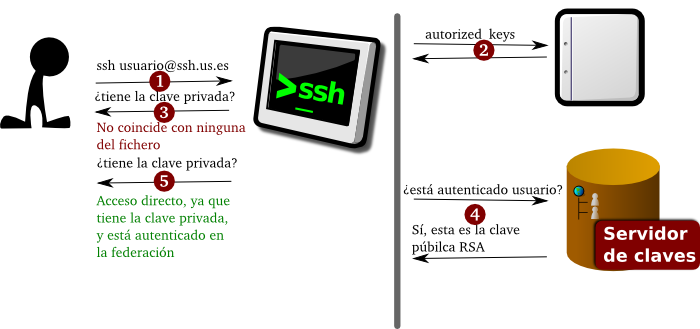
\includegraphics[width=\textwidth]{img/funcionamientossh.png}
            \caption{Funcionamiento SSH}
        \label{fig:funcionamientossh}
    \end{figure}


        \subsection{SSO para SSH, posibilidad}
    
    \section{Servidor de claves, flexibilidad, LDAP, python...}
    
    \section{Aplicación de login.}
     (posibilidad de mostrar los datos que se van a guardar en el servidor
     de claves, y pedir la autorización al usuario).

    \section{Ejemplo aplicación creación de cuentas.}
